\chapter{Theoretical background}
\label{chap:theory}

\section{Röntgenstrahlen}
\subsection*{Was sind Röntgenstrahlen und wie kann man sie im elektromagnetischen Spektrum einordnen?}
Röntgenstrahlung ist elektromagnetische Strahlung (EM-Strahlung), welche zwischen der UV-Strahlung und $\gamma$-Strahlung eingeordnet werden können.
Der typische Wellenlängenbereich für Röntgenstrahlung erstreckt sich von $100\,\text{\AA}$ bis etwa $0,05\,\text{\AA}$.
\begin{figure}[htb]
    \centering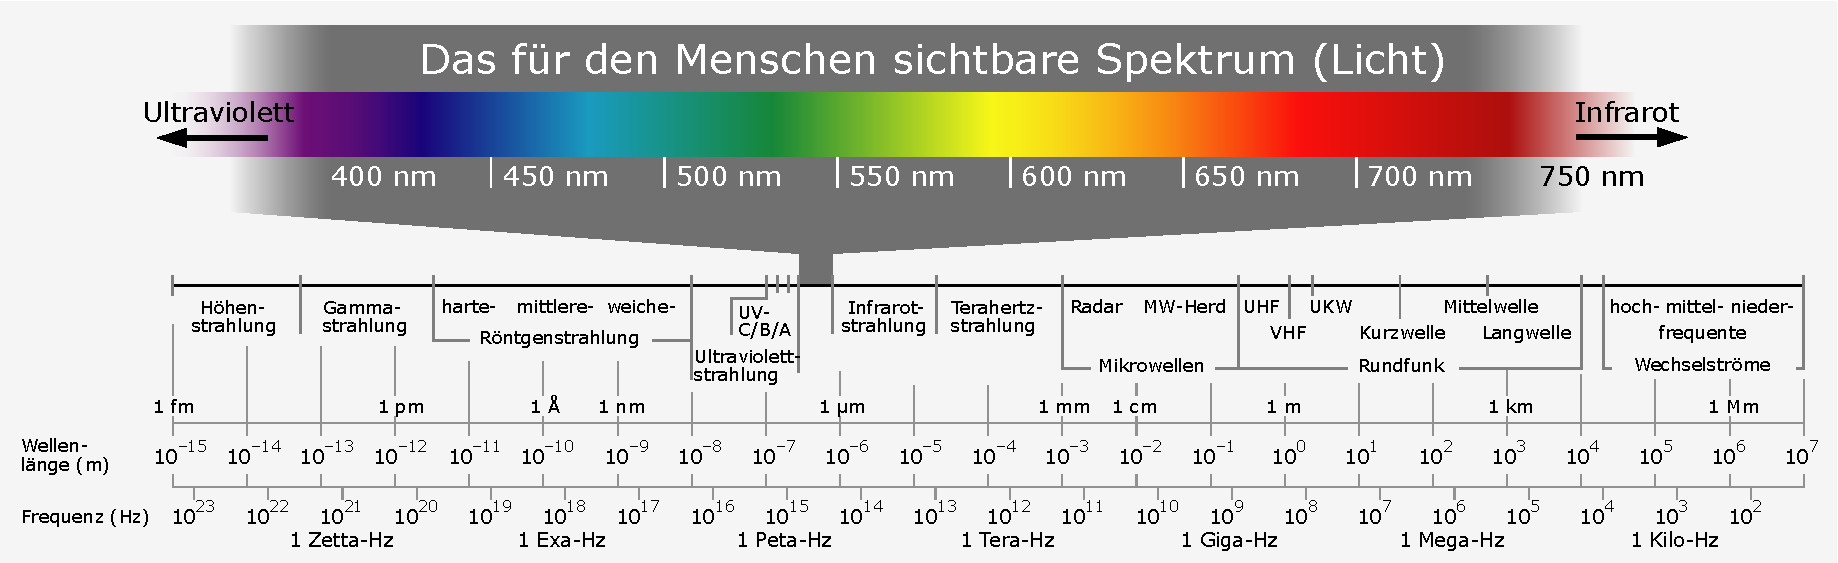
\includegraphics[width=0.9\textwidth]{Theory/Electromagnetic_spectrum_-de.pdf}
    \caption{EM-Spektrum; Röntgenstrahlung im Bereich zwischen $10\,\text{nm}$ und $5\,\text{pm}$ \cite{emspektrum}}
\end{figure}
\subsection*{Diskutieren Sie Art und Entstehung des Emissionsspektrum einer \textit{Röntgenröhre.}}
Die Röntgenröhre besteht aus einer Glühkathode und einer angeschrägten Anode.
Aus der Glühkathode emittierte Elektronen werden mittels einer großen Spannung auf die Anode beschleunigt.
Dort treffen diese auf und erzeugen Röntgenstrahlung.\\
Das Emissionsspektrum einer dieser Röhre besteht aus zwei Teilen.
Der erste Teil ist die charakteristische Strahlung, welche charakteristisch für das verwendete Anodenmaterial ist und als Spektrallinien auftreten.
Der zweite Teil ist die Bremsstrahlung, welche einen kontinuierlichen Untergrund bildet.
Sie ist unabhängig von gewählten Anodenmaterial und wird durch eine kurzwellige Grenze gekennzeichnet.\newpage
\begin{figure}[htb]
    \centering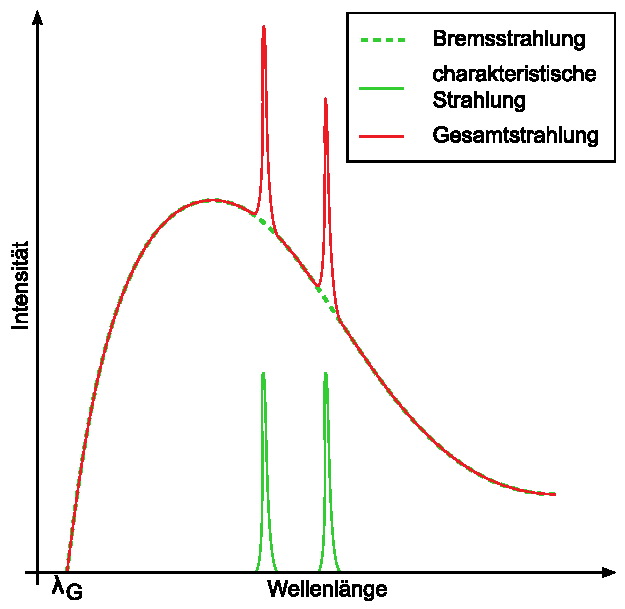
\includegraphics[width=0.4\textwidth]{Theory/emission_roehre.pdf}
    \caption{Beispielhaftes Emissionsspektrum einer Röntgenröhre \cite{emissionsspektrum}}   
\end{figure}
Die Bremsstrahlung entsteht durch die Abbremsung der in die Anode eintretenden Elektronen.
Da Elektronen mit allen Geschwindigkeiten eintreten entstehen allen Wellenlängen (Kontiuum).
Die Wellenlänge der unteren Grenze kann durch das Gesetz von Duane und Hunt berechnet werden.\\
Die charakteristische Strahlung entsteht, durch das Eindringen des Elektrons in die Anode.
Dort wird durch dieses, ein gebundenes Elektron von seinem Atom getrennt und dieser freie Platz wird von einem höhergelegenen Elektron wieder besetzt.
Das höhergelegene Elektron gibt seine überschüssige Energie in form von charakteristischer EM-Strahlung ab. \cite{EKS}
\subsection*{Wie werden Röntgenstrahlen in einem \textit{Synchrotron} erzeugt? Was passiert in einem Wiggler/Undulator?}
In einem Synchrotron werden Elektronen mittels magnetischen Feldern auf Kreisbahnen gezwungen und dort durch welchselnde elektrischen Felder beschleunigt.
Durch die Kreisbewegung erfahren die Elektronen eine Zentrifugalbeschleunigung was zu einem Energieverlust in Form von EM-Strahlung, bzw. Synchrotronstrahlung (Strahlung tangential zur Bewegungsrichtung) führt. Bei Elektronengeschwindigkeit nahe der Lichtgeschwindigkeit, liegt die abgestrahle Energie im Bereich des Röntgenspektrums. \cite{Gerthsen}\\
In einem Wiggler/Undulator wird sich dieses Phänomen, zur Erzeugung von Synchrotronstrahlung, zu nutze gemacht.
Dieser besteht aus einer Reihe Dipolmagnete, welche lenken Elektronenstrahl mit annähernd Lichtgeschwindigkeit abwechselnd nach oben und nach unten ablenken.
Durch die, bei den Richtungsänderung, herrschenden Zentrifugalkräfte wird jeweils Synchrotronstrahlung erzeugt.
Der Unterschied zwischen Wiggler und Undulator ist, dass der Wiggler ein kontinuierliches Spektrum und der Undulator ein Linienspektrum erzeugt.
Dies wird durch eine unterschiedliche Bauart erreicht.\newpage
\section{Wechselwirkung zwische Röntgenstrahlen und Materie}
\subsection*{Wie können Röntgenstrahlen und Materie wechselwirken?}
Röntgenstrahlung kann von Materie absorpiert/abgeschirmt werden.
Dies bietet die Grundlage für Röntgenstrahlabsorptionsspektroskopie.\vspace{6pt}\\
Kristalline Materie oder kleinere Strukturen können Röntgenstrahlung beugen/streuuen.
Dies ist die Grundlage für Strukturanalyse, womit die räumliche Anordnung der Atome im Kristall untersucht werden.
\subsection*{Wie und wozu können man diese jeweils in Medizin, Technik und Wissenschaft ausnutzen?}
In der Medizin wird Röntgenstrahlung zur Diagnostik (z.B. Knochenbrüche) oder zur Behandlung von speziellen Krankheiten (Bestrahlung von Krebs) eingesetzt.
In der Technik findet Röntgenstrahlung Anwendung in der Materialüberprüfung und Qualitätssicherung wieder.
Für die Wissenschaft sind Röntgenstrahlen unerlässlich um kleinste Strukturen erforschen zu können.
\section{Absorption}
\subsection*{Erläutern Sie das übliche Absorptionsgesetz für die Schwächung monochromatischer Strahlung beim Durchgang durch Materie?}
Die Abschwächung der Strahlungsleistung $P(x)$ der Röntgenstrahlung bei Absorption lässt sich wie folgt beschreiben:
\begin{equation}
    dP = -\mu P dx \Leftrightarrow P(x)=P_0e^{-\mu x}
\end{equation}
Hier ist $P_0$ die Strahlungsleistung vor Absorption, $x$ die Eindrintiefe und $\mu = \mu_S+\alpha$ der Abschwächungskoeffizient bestehent aus dem Streukoeffizient $\mu_S$ und dem Absorptionskoeffizient $\alpha$. \cite{Experimentalphysik3}\\
Der Absorption beruht auf drei Effekten: Photoeffekt (Röntgenquant wird komplett absorpiert und inneres Elektronen wird ionisiert), Compton-Effekt (Röntgenquant überträgt teilweise seine Energie auf ein fast freies Elektron in der äußeren Schale) und Paarbildung (Röntgenquant erzeugt Elektron-Positronpaar)\\
Der Absorptionskoeffizient
\begin{equation}
    \alpha=n\cdot \sigma_a
\end{equation}
kann somit als Produkt der Teilchenzahl der absorpierten Atome und deren Absorptionsquerschnitt geschrieben werden.
Experimentell findet man, dass der Absorptionsquerschnitt $\sigma_a$ gemäß
\begin{equation}
    \sigma_a=C\cdot Z^4 \cdot \lambda^3
\end{equation}
stark mit der Wellenlänge $\lambda$ der Röntgenstrahlung und der Kernladungszahl $Z$ des absorbierenden Material anwächst.
Die Konstante $C$ ist eine Absorptionsmaterial spezifische Konstante. \cite{Experimentalphysik3}
\subsection*{Warum entstehen die Absorptionskanten?}
Im Verlauf des Absorptionsquerschnitts im Abhänigkeit von der Wellenlänge finden sich Sprünge.
Diese Sprünge werden als Absorptionskanten bezeichnet und sind charakteristisch für das Absorptionsmaterial.
Die entsprechenden Energien stimmen mit den Ionisationsenergien der entsprechenden inneren Niveaus überein.\vspace{6pt}\\
Mit steigender Wellenlänge der Röntgenstrahlen können Elektronen aus immer tiefersitzenden Schalen ionisiert werden, was zum Anstieg des Absorptionsquerschnitts führt.
Dieser steigt solange an, bis man an die Ionisationsgrenze der aktuellen Schale kommt.
Danach können Elektronen der nächst tieferen Schale ionisiert werden.
Dort können aber zuerst nur Elektronen in dem obersten Niveau ionisiert werden, was zu einem Sprung im Absorptionsquerschnitts führt. \cite{Experimentalphysik3}
\subsection*{Skizzieren Sie für ein bestimmtes Element den Verlauf des Schwächungskoeffizienten \texorpdfstring{$\mu$}{U+03BC} als Funktion der Energie, \texorpdfstring{$\mu(E)$}{U+03BC(E)}, bzw. der Wellenlänge, \texorpdfstring{$\mu(\lambda)$}{U+03BC(U+03BB)}!}
Für Blei ist der Verlauf des Schwächungskoeffizienten wie folgt:
\begin{figure}[htb]
    \centering\subfigure[Energie]{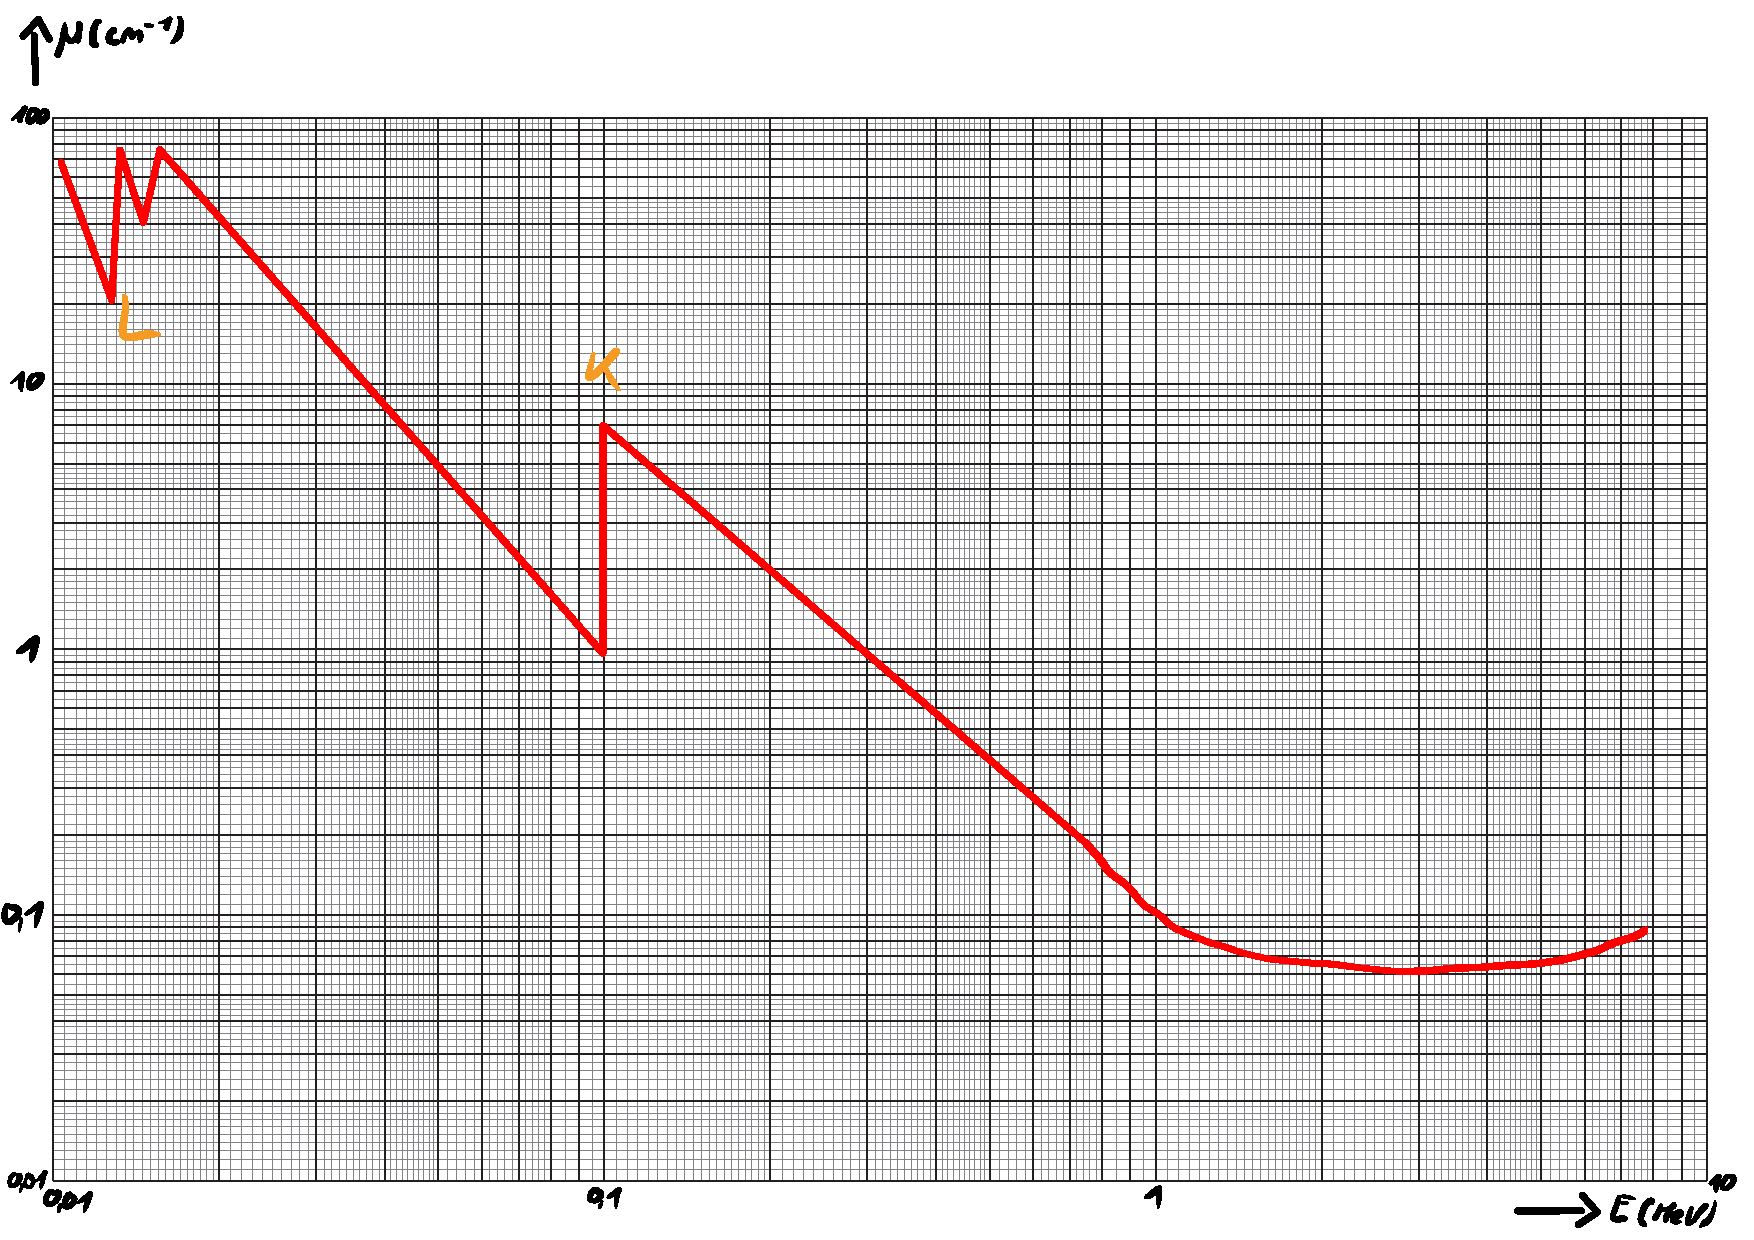
\includegraphics[width=0.47\textwidth]{Theory/Energie_genau.pdf}}
    \subfigure[Wellenlänge]{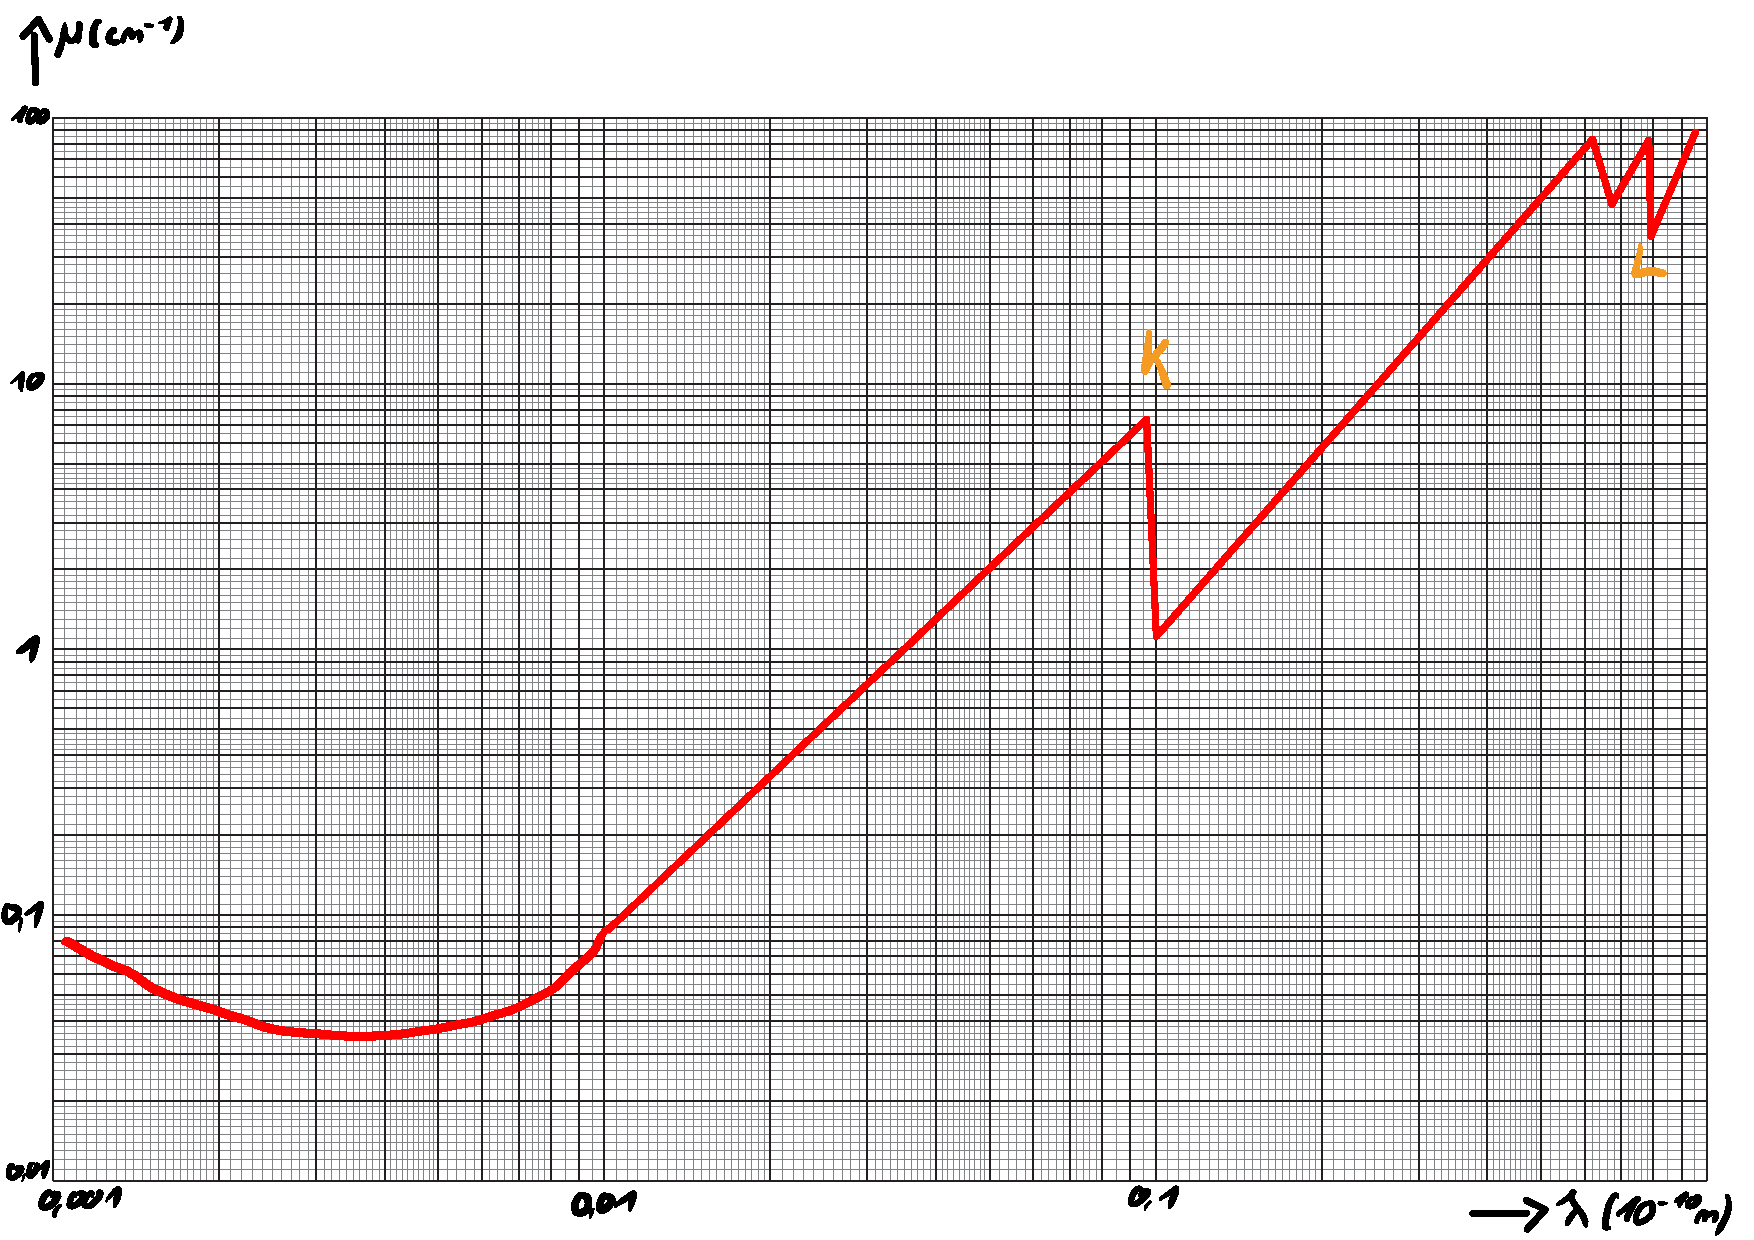
\includegraphics[width=0.47\textwidth]{Theory/Wellenlaenge_genau.pdf}}
    \caption{Schematischer Verlauf des Schwächungskoeffizienten von Blei in Abhänigkeit der Energie und Wellenlänge \cite{Krieger}}
\end{figure}\newpage
\section{Kristall und Kristallstruktur}
\subsection*{Was ist ein \textit{Kristall}? Wo gibt es Kristalle? Wo im menschlichen Körper finden sich Kristalle oder kristallines Material?}
Ein Kristall ist ein Festkörper mit einer regelmäßigen Anordnung von Atomen/Molekülen.\\
Kristalle sind sehr weit verbreitet.
Man findet sie in Salzen, Mineralien und Metallen.\\
Kristalle, bzw. kristallines Material findes sich im Körper in Form von Mineralien, Zucker und Proteinen.
\subsection*{Was versteht man unter der Kristallstruktur? Wozu mag es sinnvoll sein, die Struktur eines Materials zu kennen?}
Unter Kristallstruktur versteht man die Gesamtheit aus Translationsgitter und Atombasis. \cite{Experimentalphysik3}\\
Es ist sinnvoll die Struktur des Materials zu kennen, da es wichtig für seine Eigenschaften und Verhalten ist.
\subsection*{Was bedeutet \textit{Symmetrie} anschaulich?}
Symmetrie bezeichnet die Invarianz eines Objektes bezüglich bestimmter Operationen. \cite{Schwarzenbach}\\
Anschaulich bedeutet dies, dass man ein Objekte einer bestimmten Operation unterzieht (z.B. Drehung um die eigene Achse) und diese die selben Eigenschaften wie zuvor hat, sich also nicht verändert hat und unterscheidlich zum Ausgangszustand ist.
\subsection*{Wie ist die \textit{kubische Symmetrie} definiert und wie das \textit{kubische Gitter}? Wie hängen Symmetrie und Gitter zusammen?}
Unter kubischer Symmetrie versteht man die Gittersymmetrie eines kubischen Gitters, dieses hat die höchste Symmetrie aller Gitter da es invariant unter allen Symmetrien ist.
Unter kubischen Gitter versteht man eine Bravisgitterklasse, welche die gleichen Abstände und Winkel zwischen den äußeren Atomen einer Gitterzelle hat.\\
Das Gitter ist unter der Symmetrie invariant.
\subsection*{Wo in der \textit{Elementarzelle} sitzen die Atome?}
Die Atome sitzen immer auf den Eckpunkten der Elementarzelle (primitiv).
Zusätzlich können Sie bei einer kubischen oder orthorombischen Systemen, mittig auf den Außenflächen sitzen (flächenzentriert) oder mittig in der Zelle (raumzentriert).
Bei orthorombischen oder monoklinen Systemen ist es möglich, dass jeweils ein Atom noch mittig auf der unteren und oberen Außenfläche sitzt (basiszentriert).
\section{Beugung von Röntgenstrahlen}
\subsection*{Was versteht man unter \textit{Beugung}?}
Die Beugung ist eine typische Ausbeitungserscheinung von Wellen.
Diese weichen nach einer seitlichen Begrenzung des Wellenfeldes von einer geradlinigen Ausbreitung ab und werden abgelenkt.
Grund hierfür ist das Huygenssches Prinzip, dass jeder Punkt einer Wellenfront als Ausgangspunkt für eine neue Elementarwelle betrachtet werden kann. \cite{EKS}
\subsection*{Erklären sie, welche Bedingungen Max von Laue zur Beschreibung der Röntgenstrahlbeugung heranzog und stellen Sie kurz seinen Ansatz dar!}
Laue stellt die Bedingung, dass bei der Beugung man nur konstruktive Interferenz erhält, wenn die Änderung des Wellenvektors beim Streuprozess einem reziproken Gittervektor entspricht.
Dadurch erhält man die Richtung der beobachteten Beugungsreflexe an einem reinen Kristallgitter (ohne Verschmutzungen).\\
Der Abstand zwischen zwei Streuzentren ist der Gittervektor $\vec{R}$. Der Wellenvektor der (gestreuten) Strahlung ist ($\vec{k}'$) $\vec{k}$. Für den Gangunterschied folgt:
\begin{equation}
    \Delta x = \vec{R}\cdot\left(\frac{\vec{k}}{k}-\frac{\vec{k}'}{k'}\right)
\end{equation}
Für konstruktive Interferenz muss folgendens gelten:
\begin{equation}
    \Delta x = m\cdot\lambda\:\:m\in\mathbb{Z}
\end{equation}
Bei der elastischen Streuung ist die Wellenzahl des einfallenden und reflektieren Strahls gleich:
\begin{equation}
    k=k'=\frac{2\pi}{\lambda}
\end{equation}
Somit muss für alle $\vec{R}$ gelten:
\begin{equation}
    \vec{R}\cdot\left(\vec{k}-\vec{k}'\right)=2\pi m\:\:\text{bzw.}\:\:\exp\left[i\vec{R}\cdot\left(\vec{k}-\vec{k}'\right)\right] = 1
\end{equation}
Letzeres entspricht der Bestimmungsgleichung der reziproken Gittervektoren $\vec{K}$:
\begin{equation}
    \exp\left[i\vec{R}\cdot\vec{K}\right]=1
\end{equation}
Somit folgt die Laue-Bedingung:
\begin{equation}
    \vec{K}=\vec{k}-\vec{k}'
\end{equation}
\newpage
\subsection*{William Henry Bragg und sein Sohn William Lawrence Bragg verwendeten ein komplett anderes aber äquivalentes Modell zur Beschreibung der Röntgenstrahlbeugung. Erläutern Sie dieses! Wie lautet in diesem Kontext die Braggsche Gleichung? Welchen physikalischen Zusammenhang stelt sie dar? Erklären Sie diesen Zusammenhang anschaulich!}
Trifft Röntgenstrahlung auf einen Kristall wird ein Großteil diesen ungehindert durchdringen, ein kleiner Teil aber wird an den Atomen abgelenkt.
Diese Ablenkungen sind sehr schwach und werden stärker, wenn diese nach der Bragg-Bedingung konstruktiv interferrieren.\\
Die Braggsche Gleichung stellt die konstruktive Interferenz zwischen zwei Ebenen dar und lautet:
\begin{equation}
    n\lambda=2d\sin\left(\theta\right)
\end{equation}
Wobei $n$ ein natürliche Zahl (Beugungsordnung) ist, $\lambda$ die Wellenlänge der Röntgenstrahlung, $d$ der Abstand zwischen zwei parallelen Gitterebenen und $\theta$ der Winkel zwischen Röntgenstrahl und Gitterebene.
\subsection*{Hält man einen Einkristall in einem monochromatischen Röntgenstrahl, so "passiert normalerweise nichts". Welche Bedingung muss erfüllt sein, damit ein Beugungsreflex entsteht? Welche beiden Parameter kann man nun variieren, damit man an diesem Einkristall einen Beugungsreflex erfassen kann?}
Es muss die Bragg-Bedingung er füllt ein, um einen Beugungsreflex zu bekommen.
Entweder man änder die Wellenlänge der Röntgenquelle oder man verdreht den Kristall, damit die Bragg-Bedinung erfüllt wird.
\section{Zentriertes Gitter}
\subsection*{Was versteht man unter einem \textit{zentrierten Gitter}? Diskutieren Sie kurz die verschiedenen Möglichkeiten der Gitterzentrierung und geben Sie auch an, wie viele Gitterpunkte dann jeweils pro Elementarzelle vorliegen. Geben Sie die Koordinaten dieser äquivalenten Gitterpunkte pro Elementarzelle an.}
In einem zentrierten Gitter finden sich, im Gegensatz zum primitiven Gitter welches nur Gitterpunkte an den Ecken hat, weitere Punkte in der Elementarzelle.
Man unterscheidet zwischen raumzentrierten Gitter, dort findet sich ein weiterer Gitterpunkt mitten in der Elementarzelle.
Somit liegen in der Zelle insgesamt zwei Atome.
Die Gittervektoren des bcc-Gitters (base-centered-cubic) lauten: $\vec{a}=\frac{a}{2}\left(-1,1,1\right)\:\:\vec{b}=\frac{a}{2}\left(1,-1,1\right)\:\:\vec{c}=\frac{a}{2}\left(1,1,-1\right)$\\.
Ein weiteres zentriertes Gitter ist das flächenzentrierte Gitter, dort ist mittig in jeder Seitenfläche ein weiteres Atom.
In der Elementarzelle sind somit 4 Atome.
Die Gittervektoren des fcc-Gitters (face-centered-cubic) lauten: $\vec{a}=\frac{a}{2}\left(0,1,1\right)\:\:\vec{b}=\frac{a}{2}\left(1,0,1\right)\:\:\vec{c}=\frac{a}{2}\left(1,1,0\right)$\\.
Das letzte zentrierte Gitter ist das Basiszentrierte Gitter, welches jeweils mittig auf der Ober- und Unterseite noch ein Atom sitzen hat.
Es finden sich insgesamt 2 Atome in der Einheitszelle.
Die Gittervektoren des basiszentrierten orthorombischen Gitters sind: $\vec{a}=\left(0,0,c\right)\:\:\vec{b}=\left(\frac{a}{2},\frac{b}{2},0\right)\:\:\vec{c}=\left(-\frac{a}{2},\frac{b}{2},0\right)$
\subsection*{Wie und warum entstehen bei zentrierten Gittern im Beugungsbild \textit{systematische Auslöschungen}? Wie lauten diese Auslöschungsregeln?}
Durch das zentrierte Bravisgitter kommt es zu einer destruktiven Interferenz des zusätzlichen Atoms.
Diese tritt auf, wenn von den Miller'schen/Laue-Indizes $hkl$ die Summe aus $h$ und $k$ ungerade ist. \cite{UniFreiburg}
\section[Beschreibung eines Peaks im Pulverdiffraktogramm]{Ein \textit{Peak} im \textit{Pulverdiffraktogramm} lässt sich durch seien Form (Profil), seine Lage \texorpdfstring{($2\theta$)}{2(U+03B8)} und seine Fläche (Intensität) beschreiben.}
\subsection*{Was kann man aus den Peaklagen bestimmen?}
Aus den Peaklagen ($2\theta$) lässt sich die der Gitterebenen Abstand des Kristalls bestimmen.
\subsection*{Was kann man aus den Peakintensitäten bestimmen?}
Durch die Intensitäten können die Anordnung der Atome auf einer Gitterebene (somit das Bravisgitter) bestimmt werden.
\subsection*{Welche Faktoren bestimmen das Profil? Was versteht man hierbei unter \textit{axialer Divergenz}?}
Unter axialer Divergenz versteht man Einflüsse durch optische Elemente (Blenden, etc.) auf den Strahl. \cite{Kleber}
\subsection*{Was bedeuten \textit{Atomformfaktor} und \textit{Strukturfaktor} anschaulich?}
Der Atomformfaktor ist ein Maß für die Winkelabhängigkeit der Intensität der gestreuten Strahlung.
Anschaulich spiegelt er die Anzahl der unter einen bestimmten Winkel an der Streuung beteiligten Elektronen wieder.\\
Der Strukturfaktor bezieht nun die Wechselwirkung aller Atome in der Elementarzelle mit ein und spiegelt die Gesamtbeugung an dem Gitter wieder.
\subsection*{Wie kann man die Intensität berechnen? Was bedeuten in diesem Zusammenhang die Begriffe \textit{Absorptions-}, \textit{Lorentz-}, \textit{Polarisations-}, \textit{Extinktions-} und \textit{Flächenhäufigkeitsfakor}?}
Die (theoretische) Intensität ist proportional zu dem Quadrat des Betrages des Strukturfaktors des Reflexes.
Der Proportionalitätsfaktor beinhaltet die Ursprungsintensität $I_0$, die Wellenläge des Primarstrahls $\lambda$ und Korrekturfaktoren. \cite{Kleber}
Der Absorptionsfaktor berücksichtigt, dass ein Teil der Röntgenstrahlung absorpiert und somit nicht gebeugt wird.\\
Durch den Lorentzfaktor wird berücksichtigt, dass bei bewegten Kristallen Reflexe mit höheren Beugungswinkel länger in Reflexionsstellung bleiben als welche mit niedrigem.
Aufgrund der Bewegung nimmt scheinbar die Intensität der höheren Beugungswinkel zu.\\
Der Polarisationsfaktor berücksichtigt, dass die Amplitude der gestreuten Strahlung proportional zum Sinus des Winkels zwischen der Orientierung des elektrischen Vektors der einfallenden und der gestreuten Strahlung ist.
Dieser ist bei unpolarisierter Röntgenstrahlung wichtig.\\
Durch den Extinktionsfaktor wird berücksichtigt, dass mit zunehmender Eindrintiefe die Strahlung durch Braggstreuung abgeschwächt wird.\\
Der Flächenhäufigkeitsfakor berücksichtigt die Überhöhung der Intensität eines Reflexes, da mehrere Netzebenenscharen mit den selben Mitterschen Indizes gleichzeitig in Reflexionsstellung befinden. \cite{Kleber} 
\subsection*{Was beschreibt der \textit{Temperaturfaktor} (Debye-Waller-Faktor) und wie wirkt er sich auf die Intensität der Reflexe aus?}
Durch den Temperaturfaktor wird die Zunahme der Auslenkungen der Schwingungen der Atoma um ihre Gleichgewichtslage bei zunehmender Temperatur berücksichtigt.
Die Zunahme der Schwingungen führt zu einer Abnahme der Streukraft und der Intensitäten der Reflexe.
\subsection*{Aus welchen Komponenten setzt sich der Untergrund in einem Pulverdiffraktogramm zusammen? Warum ist der Unterschied bei niedrigen Winkeln oft viel höher?}
Der Untergrund kommt aus Fremdwellenlängenanteilen der monochromatischen Röntgenstrahlung zustande.
Fremdkörper im Strahlengang oder der Probe gehören ebenfalls zum Untergrund.
Bei kleineren Winkel ist können breits kleinere Abweichungen in der Wellenlänge dazu führen, dass weiter Reflexe auftreten als bei größeren Winkeln.